\documentclass[a4paper,10pt]{article}
%\documentclass[a4paper,10pt]{scrartcl}

\usepackage{../mystyle}

\setromanfont[Mapping=tex-text]{Linux Libertine O}
% \setsansfont[Mapping=tex-text]{DejaVu Sans}
% \setmonofont[Mapping=tex-text]{DejaVu Sans Mono}

\title{\sc Einführung in die Komplexe Analysis \\ \Large Blatt 2}
\author{Jendrik Stelzner}
\date{\today}

\begin{document}
\maketitle





\section{(Konjugierte Nullstellen)}
Bekanntermaßen handelt es sich bei der Konjugation $\C \to \C, x+iy \to x-iy$ um einen $\R$-Algebraauto\-morph\-ismus von $\C$ (dem einzigen neben der Identität $\id_\C$). Inbesondere ist $\bar{x} = x$ für alle $x \in \R$. Es ist daher für alle $\rho \in \C$
\[
 \overline{P(\rho)} = \overline{\sum_{k=0}^n a_k \rho^k} = \sum_{k=0}^n a_k \bar{\rho}^k = P(\bar{\rho}).
\]
Also ist für alle $\rho \in \C$
\[
 0 = P(\rho) \Leftrightarrow 0 = \overline{P(\rho)} \Leftrightarrow 0 = P(\bar{\rho}).
\]





\section{(Niveaulinien komplexwertiger Funktionen)}
Für $z = x+iy \in \C$ ist
\[
 z^2 = (x+iy)^2 = x^2 - y^2 + i2xy,
\]
also
\[
 \Re\left(z^2\right) = x^2-y^2 \text{ und } \Im\left(z^2\right) = 2xy.
\]

Für die Niveaulinie von $\Re\left(z^2\right)$ für $c \in \R$ ergibt sich, dass $x^2-y^2 = c$ für $x^2 < c$ keine Lösung besitzt, und sonst, dass $y = \pm \sqrt{x^2-c}$. Für die Niveulinienen von $\Im\left(z^2\right) = 2xy$ ergibt sich für $c=0$ die Vereinigung von reeler und imaginärer Achse, und $y = 2/(cx)$ für $c \neq 0$. Für ein Bild der Niveulinien siehe Abbildung \ref{fig: Niveaulinien z²} auf Seite \pageref{fig: Niveaulinien z²}.
\begin{figure}\centering
 % nun kommt ziemlich hässlicher Code, den ich bei Gelegenheit gegen etwas besseres austauschen sollte
 \newcommand{\samplerate}{400}
 \begin{tikzpicture}[scale=0.2, domain=-10:10]
  % die Koordinatenachsen
  \draw[very thick,->] (-10,0) -- (10,0) node[anchor=west] {$\Re(z)$}; % Re-Achse
  \draw[very thick,->] (0,-10) -- (0,10) node[anchor=south] {$\Im(z)$}; % Im-Achse
  % Niveulinien für
  % c = 0
  \draw plot function {x};
  \draw plot function {-x};
  % c = -5
  \draw plot function {sqrt(x**2+5)};
  \draw plot function {-sqrt(x**2+5)};
  % c = 5
  \draw[domain=sqrt(5):10,smooth,samples=\samplerate] plot function {sqrt(x**2-5)};
  \draw[domain=sqrt(5):10,smooth,samples=\samplerate] plot function {-sqrt(x**2-5)};
  \draw[domain=-10:-sqrt(5),smooth,samples=\samplerate] plot function {sqrt(x**2-5)};
  \draw[domain=-10:-sqrt(5),smooth,samples=\samplerate] plot function {-sqrt(x**2-5)};
  % c = -15
  \draw plot function {sqrt(x**2+15)};
  \draw plot function {-sqrt(x**2+15)};
  % c = 15
  \draw[domain=sqrt(15):10,smooth,samples=\samplerate] plot function {sqrt(x**2-15)};
  \draw[domain=sqrt(15):10,smooth,samples=\samplerate] plot function {-sqrt(x**2-15)};
  \draw[domain=-10:-sqrt(15),smooth,samples=\samplerate] plot function {sqrt(x**2-15)};
  \draw[domain=-10:-sqrt(15),smooth,samples=\samplerate] plot function {-sqrt(x**2-15)};
 \end{tikzpicture}
 \begin{tikzpicture}[scale=0.2, domain=-10:10]
  % die Koordinatenachsen
  \draw[very thick,->] (-10,0) -- (10,0) node[anchor=west] {$\Re(z)$}; % Re-Achse
  \draw[very thick,->] (0,-10) -- (0,10) node[anchor=south] {$\Im(z)$}; % Im-Achse
  % Niveulinien für
  % c = 4
  \draw[domain=0.2:10,smooth,samples=\samplerate] plot function {2/x};
  \draw[domain=-10:-0.2,smooth,samples=\samplerate] plot function {2/x};
  % c = -4
  \draw[domain=0.2:10,smooth,samples=\samplerate] plot function {-2/x};
  \draw[domain=-10:-0.2,smooth,samples=\samplerate] plot function {-2/x};
  % c = 16
  \draw[domain=0.8:10,smooth,samples=\samplerate] plot function {8/x};
  \draw[domain=-10:-0.8,smooth,samples=\samplerate] plot function {8/x};
  % c = -16
  \draw[domain=0.8:10,smooth,samples=\samplerate] plot function {-8/x};
  \draw[domain=-10:-0.8,smooth,samples=\samplerate] plot function {-8/x};
 \end{tikzpicture}
 \caption{Niveulinien von $\Re\left(z^2\right)$ (links) und $\Im\left(z^2\right)$ (rechts).}
 \label{fig: Niveaulinien z²}
\end{figure}

Für $z = x+iy \in \C$ ist
\[
 \frac{1}{z} = \frac{1}{x+iy} = \frac{x}{x^2+y^2} + i\frac{-y}{x^2+y^2},
\]
also
\[
 \Re\left(\frac{1}{z}\right) = \frac{x}{x^2+y^2} \text{ und }
 \Im\left(\frac{1}{z}\right) = \frac{-y}{x^2+y^2}.
\]

Um die Niveulinien von $\Re(f)$ für $f : \C \smallsetminus \{0\} \to \C \smallsetminus \{0\}, z \mapsto z^{-1}$ zu bestimmen, bemerken wir zunächst, dass $f$ involutiv ist. Es ist daher für alle $c \in \R$ und $z \in \C \smallsetminus \{0\}$
\begin{align*}
 \Re(f(z)) = c
 &\Leftrightarrow f(z) \in \{c + i\lambda : \lambda \in \R\} \smallsetminus \{0\} \\
 &\Leftrightarrow z \in f^{-1}(\{c + i\lambda : \lambda \in \R\} \smallsetminus \{0\}) \\
 &\Leftrightarrow z \in f(\{c + i\lambda : \lambda \in \R\} \smallsetminus \{0\}).
\end{align*}
Wir bestimmen also $f(\{c+i\lambda : \lambda \in \R\} \setminus \{0\})$. Für $c = 0$ erhalten wir so, dass
\[
 \Re(f(z)) = 0 \Leftrightarrow z \in i\R \setminus\{0\}.
\]

Wir behaupten, dass für $c \in \R, c \neq 0$
\[
 f(\{c + i\lambda : \lambda \in \R\})
 = \left\{z \in \C \smallsetminus \{0\} : \left|z-\frac{1}{2c}\right| = \frac{1}{2|c|} \right\}.
\]
Dies ergibt sich daraus, dass die Abbildung $\R \to S^1 \smallsetminus\{1\}, \lambda \to (i\lambda+1)/(i\lambda-1)$ eine Bijektion ist, und für $c \in \R, c \neq 0$.
\begin{align*}
 &\,f(\{c+i\lambda : \lambda \in \R\})
 = f(\{c-i\lambda : \lambda \in \R\})
 = \left\{\frac{1}{c-i\lambda} : \lambda \in \R\right\} \\
 =&\, \left\{\frac{1}{c-i\lambda} - \frac{1}{2c} : \lambda \in \R\right\} + \frac{1}{2c}
 = \left\{\frac{c+i\lambda}{2c(c-i\lambda)} : \lambda \in \R\right\} + \frac{1}{2c} \\
 =&\, -\frac{1}{2c} \left\{\frac{i\lambda+c}{i\lambda-c} : \lambda \in \R\right\} + \frac{1}{2c}
 = -\frac{1}{2c} \left\{\frac{i\frac{\lambda}{c}+1}{i\frac{\lambda}{c}-1} : \lambda \in \R\right\} + \frac{1}{2c} \\
 =&\, -\frac{1}{2c} \left\{\frac{i\lambda+1}{i\lambda-1} : \lambda \in \R\right\} + \frac{1}{2c}
 = -\frac{1}{2c} \left(S^1 \smallsetminus\{1\}\right) + \frac{1}{2c} \\
 =&\, \left\{z \in \C \setminus\{0\} : \left|z-\frac{1}{2c}\right| = \frac{1}{2|c|}\right\}.
\end{align*}
Die Niveulinien von $\Re(1/z)$ sind also die imaginäre Achse ohne $0$ und die Kreise mit Radius $1/(2|c|)$ um den Mittelpunkt $1/(2c)$ für $c \in \R, c \neq 0$.

Für die Niveulinien von $\Im(1/z)$ bemerken wir, dass $\Im(1/z) = \Re(1/(iz))$. Die Niveulinien von $\Im(1/z)$ ergeben sich also aus denen von $\Re(1/z)$ durch Rotation um $\pi/2$.

Skizziert sehen die Niveulinien aus wie in Abbildung \ref{fig: Niveulinien von 1/z} auf Seite \pageref{fig: Niveulinien von 1/z}.

\begin{figure}\centering
 \newcommand{\samplerate}{0}
 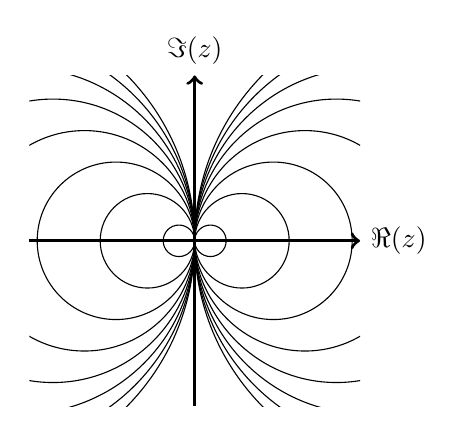
\begin{tikzpicture}[scale=0.2]
  % die Koordinatenachsen
  \draw[very thick,->] (-10.5,0) -- (10.5,0) node[anchor=west] {$\Re(z)$}; % Re-Achse
  \draw[very thick,->] (0,-10.5) -- (0,10.5) node[anchor=south] {$\Im(z)$}; % Im-Achse
  % Niveulinien
  \begin{scope}
   \clip (-10.5,-10.5) rectangle (10.5,10.5);
   \foreach \r in {-15, -13, ..., 13, 15}
    \draw (\r,0) circle (\r);
  \end{scope}
 \end{tikzpicture}
 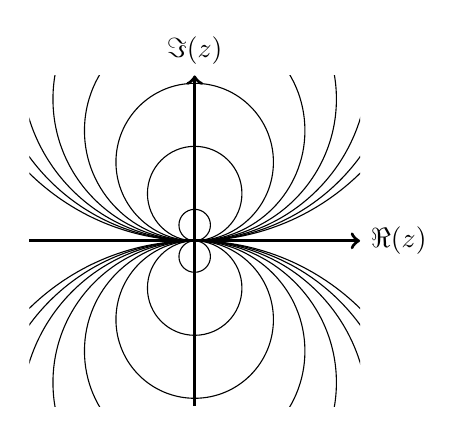
\begin{tikzpicture}[scale=0.2]
  % die Koordinatenachsen
  \draw[very thick,->] (-10.5,0) -- (10.5,0) node[anchor=west] {$\Re(z)$}; % Re-Achse
  \draw[very thick,->] (0,-10.5) -- (0,10.5) node[anchor=south] {$\Im(z)$}; % Im-Achse
  % Niveulinien
  \begin{scope}
   \clip (-10.5,-10.5) rectangle (10.5,10.5);
   \foreach \r in {-15, -13, ..., 13, 15}
    \draw (0,\r) circle (\r);
  \end{scope}
 \end{tikzpicture}
 \caption{Niveulinien von $\Re(1/z)$ (links) und $\Im(1/z)$ (rechts).}
 \label{fig: Niveulinien von 1/z}
\end{figure}





\section{(Real- und Imaginärteil quadratischer Funktionen)}
Wir behaupten, dass $p(x,y) = ax^2 + bxy + cy^2$ mit $a,b,c \in \R$ genau dann Realteil eines komplexen Polynoms $P$ der Form $P(z) = Az^2 + Bz + C$ mit $A,B,C \in \C$ ist, wenn $c = -a$.

Ist $c = -a$, so ist für beliebiges $b \in \R$
\[
 p(x,y) = ax^2 + bxy - ay^2 = \Re\left(\left(a-\frac{1}{2}bi\right)(x+iy)^2\right).
\]

Sei andererseits $p = \Re(P)$ für ein komplexes Polynom $P$ wie oben. Da
\[
 \Re(C) = \Re(P(0)) = p(0,0) = 0
\]
ist $p = \Re(Az^2+Bz)$, wir können also o.B.d.A. davon ausgehen, dass $C=0$. Da für alle $z = x+iy \in \C$
\begin{align*}
 0 &= p(x,y) - p(-x,-y) = \Re(P(z))-\Re(P(-z)) \\
   &= \Re(P(z)-P(-z)) = \Re(Bz - B(-z)) = \Re(2Bz) = 2 \Re(Bz)
\end{align*}
ist $\Re(Bz) = 0$ für alle $z \in \C$. Da $0 = \Re(B \bar{B}) = \Re(|B|^2)= |B|^2$ folgt, dass $B = 0$. Also ist $P(z) = Az^2$ für $A = x_A + iy_A \in \C$. Es ist daher
\[
 p(x,y) = \Re(Az^2) = \Re((x_A+iy_A)(x+iy)^2) = x_Ax^2 - 2y_Axy - x_A y^2,
\]
was die Behauptung zeigt.

Man bemerke noch, dass $p$ genau dann Imaginärteil eines komplexen Polynoms vom Grad $n$ ist, wenn $p$ Realteil eines komplexen Polynoms vom Grad $n$ ist, denn $p = \Im(P) \Leftrightarrow p = \Re(-iP)$, bzw. $p = \Re(P) \Leftrightarrow p = \Im(iP)$ für jedes komplexe Polynom $P$. Also ist $p$ genau dann Imaginärteil eines passenden 2komplexen Polynoms $P$ der Form $P(z) = Az^2+Bz+C$ mit $A,B,C \in \C$, wenn $a = -c$.





\section{Betrag der Exponentialabbildung}
Für alle $z \in \C$ ist
\[
 |e^z| = \left|e^{\Re(z)+i\Im(z)}\right| = \left|e^{\Re(z)} e^{i\Im(z)}\right|
 = \left|e^{\Re(z)}\right| \left|e^{i\Im(z)}\right| = e^{\Re(z)}.
\]





\section{(Der Sinus im Komplexen)}
Wir bemerken zunächst, dass für alle $z = x+iy \in \C$
\begin{align*}
 \sin(x+iy)
 &= \frac{e^{i(x+iy)}-e^{-i(x+iy)}}{2i}
 = \frac{e^{-y} e^{ix} - e^y e^{-ix}}{2i} \\
 &= \frac{e^{-y}-e^y}{2i} \cos(x) + i \frac{e^{-y}+e^y}{2i} \sin(x) \\
 &= \cosh(y) \sin(x) + i \sinh(y) \cos(x). \tag{1}\label{eq: sin umgeformt}
\end{align*}
Es sei nun
\begin{gather*}
 S^+ := \left\{z \in \C : \Re(z) = \frac{\pi}{2}, \Im(z) \geq 0\right\}
      = \left\{\frac{\pi}{2} + \lambda i : \lambda \in \R, \lambda \geq 0\right\}, \\
 S^- := \left\{z \in \C : \Re(z) = -\frac{\pi}{2}, \Im(z) \leq 0\right\}
      = \left\{-\frac{\pi}{2} + \lambda i : \lambda \in \R, \lambda \leq 0\right\},
\shortintertext{sowie}
 T := \left\{z \in \C : |\Re(z)| < \frac{\pi}{2}\right\}
    = \left\{x + iy : x \in \left(-\frac{\pi}{2},\frac{\pi}{2}\right), y \in \R \right\}.
\end{gather*}
Da für alle $\pi/2 + i\lambda \in S^+$
\[
 \sin\left(\frac{\pi}{2} + i\lambda\right)
 = \sin\left(\frac{\pi}{2}\right) \cos(i\lambda) + \sin(i\lambda)\cos\left(\frac{\pi}{2}\right)
 = \cos(i\lambda)
 = \cosh(\lambda)
\]
und $\cosh : [0,\infty) \to [1,\infty)$ bijektiv ist, ist $\sin : S^+ \to [1,\infty) \subseteq \R$ bijektiv. Analog ist für alle $\pi/2 + i\lambda \in S^-$
\[
 \sin\left(-\frac{\pi}{2} + i\lambda\right)
 = -\cosh(\lambda),
\]
also $\sin: S^- \to (-\infty, -1] \subseteq \R$ bijektiv.

Um die Bijektivität $\sin : S^+ \cup S^- \cup T \to \C$ zu zeigen, genügt es nun zu zeigen, dass
\[
 \sin : T \to \C \smallsetminus ( (-\infty,-1] \cup [1,\infty)) =: A
\]
bijektiv ist.

Hierfür bemerken wir zunächst, dass tatsächlich $\sin z \in A$ für alle $x+iy = z \in T$, denn da $x \in (-\pi/2, \pi/2)$ ist $\Re(\sin z) = \sin(x) \in (-1,1)$ für $y = 0$ und $\Im(z) \neq 0$ für $y \neq 0$.

Als Nächstes zeigen wir, dass $\sin : T \to A$ injektiv ist. Seien $x+iy, x'+iy' \in T$ mit $\sin(x+iy) = \sin(x'+iy')$.

Ist $x \neq x'$ und $y \neq y'$, so bemerken wir zunächst, dass aus \eqref{eq: sin umgeformt} folgt, dass
\begin{align*}
 \sgn(x) = \sgn(\cosh(y)\sin(x)) &= \sgn(\cosh(y')\sin(x')) = \sgn(x') \text{ und} \\
 \sgn(y) = \sgn(\sinh(y)\cos(x)) &= \sgn(\sinh(y')\cos(x')) = \sgn(y').
\end{align*}
Es muss also bereits $|x| \neq |x'|$ und $|y| \neq |y'|$. Wir können dabei o.B.d.A. davon ausgehen, dass $|x| < |x'|$. Da daher $|\sin(x)| < |\sin(x')|$ folgt aus
\[
 \cosh(y)|\sin(x)| = \cosh(y')|\sin(x')|,
\]
dass $\cosh(y) > \cosh(y')$, also $|y| > |y'|$. Aus $|x| < |x'|$ und $|y| > |y'|$ folgt, dass $|\sinh(y)| > |\sinh(y')|$ und $\cos(x) > \cos(x')$, also
\[
 |\sinh(y)|\cos(x) > |\sinh(y')|\cos(x').
\]
Dies steht wegen \eqref{eq: sin umgeformt} im Widerspruch zu $\sin(x+iy)=\sin(x'+iy')$. Es muss also $x = x'$ oder $y = y'$.

Ist $x = x'$, so folgt aus \eqref{eq: sin umgeformt}, dass $\sinh y  = \sinh y'$ (da $\cos(x) = \cos(x') \neq 0$), also $y = y'$ (denn $\sinh : \R \to \R$ ist bijektiv). Ist $y = y'$, so folgt aus \eqref{eq: sin umgeformt}, dass $\sin(x) = \sin(x')$ (denn $\cosh y = \cosh y' \neq 0$), also $x = x'$ (denn $\sin (-\pi/2,\pi/2) \to (-1,1)$ ist bijektiv).

Dass zeigt, dass für $x+iy, x'+iy' \in T$ mit $\sin(x+iy) = \sin(x'+iy')$ bereits $x=x'$ und $y=y'$, also $x+iy = x'+iy'$. Das zeigt, dass $\sin : T \to A$ injektiv ist.

Zuletzt zeigen wir, dass $\sin : T \to A$ surjektiv ist, also $A = \sin(T)$. Indem man $x=0$, bzw. $y=0$ fest wählt, wird aus \eqref{eq: sin umgeformt} klar, dass $i\R \in \sin(T)$, bzw. $(-1,1) \in \sin(T)$. Aus \eqref{eq: sin umgeformt} ergibt sich auch direkt, dass $\sin(\bar{z}) = \overline{\sin z}$ und $\sin(-z) = -\sin z$ für alle $z \in \C$. Da $T$ unter $z \mapsto -z$ und $z \mapsto \bar{z}$ abgeschlossen ist, genügt es daher zum Nachweis der Surjektivität zu zeigen, dass $A' \subseteq \sin(T)$ für
\[
 A' = \{z \in A : \Re(z), \Im(z) > 0\} = \{x+iy : x,y \in (0,\infty)\}.
\]

Sei $z \in A'$ beliebig aber fest. Man bemerke, dass $|z| > 0$ und $\arg(z) \in (0,\pi/2)$. Für $y > 0$ betrachten wir die Abbildung
\[
 \varphi_y : \left[0,\frac{\pi}{2}\right] \to \C, x \to \sin(x+iy) = \cosh(y)\sin(x)+i\sinh(y)\cos(x).
\]
Offenbar ist $\varphi_y(0) = i\sinh(y)$ und $\varphi_y(\pi/2) = \cosh(y)$. Insbesondere ist daher
\[
 \arg(\varphi_y(0)) = \frac{\pi}{2} \text{ und } \arg\left(\varphi_y\left(\frac{\pi}{2}\right)\right) = 0,
\]
wobei klar ist, dass $\arg \circ \varphi_y : [0,\pi/2] \to [0,\pi/2]$ stetig und streng monoton fallend ist. Insbesondere gibt es daher ein eindeutiges $x_y \in (0,\pi/2)$ mit $\arg(\varphi_y(x_y)) = \arg(z)$, wobei klar ist, dass $x_y$ stetig von $y$ abhängt.

Wir bemerken, dass $\sinh(y) \leq |\varphi_y(x)| \leq \cosh(y)$ für alle $y > 0$ und $x \in [0,\pi/2]$, da nach \eqref{eq: sin umgeformt}
\[
 |\varphi_y(x)| = \sqrt{\cosh^2(y)\sin^2(x)+\sinh^2(y)\cos(x)}
\]
und
\begin{align*}
  &\,\sqrt{\cosh^2(y)\sin^2(x)+\sinh^2(y)\cos^2(x)} \\
 =&\, \sqrt{(1+\sinh^2(y))\sin^2(x)+\sinh^2(y)\cos^2(x)} \\
 =&\, \sqrt{\sin^2(x)+\sinh^2(y)}
 \geq \sinh(y)
\end{align*}
sowie
\begin{align*}
  &\,\sqrt{\cosh^2(y)\sin^2(x)+\sinh^2(y)\cos^2(x)} \\
 =&\, \sqrt{\cosh^2(y)\sin^2(x)+(\cosh^2(y)-1)\cos^2(x)} \\
 =&\, \sqrt{\cosh^2(y)-\cos^2(x)}
 \leq \cosh(y).
\end{align*}
Insbesondere gibt es daher $0 < y_- < y_+$, so dass
$
 |\varphi_{y_-}\left(x_{y_-}\right)| < |z| <  |\varphi_{y_+}\left(x_{y_+}\right)|.
$
Da $x_y$ stetig von $y$ abhängt, und damit auch $|\varphi_y(x_y)|$, gibt es daher nach dem Zwischenwertsatz ein $y_- < y_0 < y_+$ mit $|\varphi_{y_0}\left(x_{y_0}\right)| = |z|$. Da nach Konstruktion auch $\arg\left(\varphi_{y_0}\left(x_{y_0}\right)\right) = \arg(z)$ folgt damit, dass
$
 \varphi_{y_0}\left(x_{y_0}\right) = \sin(x_{y_0}+iy_0) = z.
$
Da $x_{y_0} \in (0,\pi/2)$ und $y_0 > 0$, also $x_{y_0}+iy_0 \in T$, zeigt dies, dass $A' \subseteq \sin(T)$, und damit die Surjektivität von $\sin : T \to A$.





\end{document}
